% SC3270 --- Chapter 7: Separation Logic - Reasoning About Heap and Pointers (0->100 ground-up)
\chapter{Separation Logic: Reasoning About Heap and Pointers}
\label{ch:separation}

\begin{quote}
\emph{``A program without pointers is a house without rooms; a logic without {\large$*$} is a map without walls.''} Separation logic adds the walls back so you can reason about one room at a time.
\end{quote}

\noindent\fbox{\parbox{\dimexpr\linewidth-2\fboxsep-2\fboxrule}{%
\textbf{From zero: no separation logic assumed.} We start from why ordinary Hoare logic stumbles on aliasing, build the heap model, introduce separating conjunction and its rules, and prove tiny heap programs. Only basic pointers and Hoare triples are assumed.}}
\vspace{0.4em}

\section*{Learning Outcomes}
After this chapter you will be able to:
\begin{enumerate}[label=(L\arabic*)]
    \item explain why aliasing breaks the Hoare assignment axiom;
    \item define heap, heaplet, and the satisfaction of points-to $x\mapsto v$;
    \item use separating conjunction $*$ and $\text{emp}$ to describe disjoint heaps;
    \item apply the heap axioms (lookup, mutate, new, dispose) and the frame rule;
    \item specify list segments and prove in-place list reversal sketch.
\end{enumerate}

% ============================================================
\section{Why Hoare Logic Stumbles on the Heap}
\label{sec:aliasing}
\paragraph{Intuition.} Ordinary assertions like $x=5$ describe the \emph{store} (variables). They have no language for ``the heap cell at address $x$ holds $5$''. Worse, aliasing means two names can denote the same cell: after $y:=x$, writing through $y$ changes what you read through $x$. The Hoare assignment axiom $Q[x\mapsto e]$ assumes variables are distinct names for distinct slots; for heap writes $[x]:=e$ that assumption is false when $x$ and $y$ alias.

\begin{example}[Aliasing counterexample]
\[
\{x\mapsto 0 * y\mapsto 0\}\; [x]:=3\; \{x\mapsto 3 * y\mapsto 0\}
\]
is claimed. But if $x=y$ (same address), after $[x]:=3$ we have $x\mapsto3 * y\mapsto3$ (they are the same cell!), so the post claiming $y\mapsto0$ is false. Ordinary conjunction $x\mapsto0\land y\mapsto0$ does not preclude $x=y$; we need a connective that \emph{forces} disjointness. That is $*$.
\end{example}

\begin{figure}[h]\centering
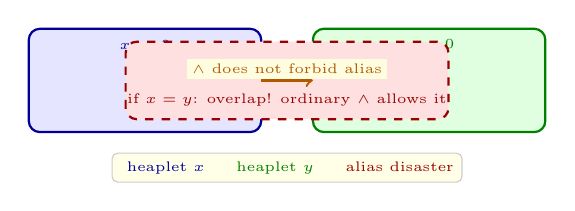
\begin{tikzpicture}[scale=0.82,font=\scriptsize]
\draw[fill=blue!10,draw=blue!60!black,thick,rounded corners=4pt] (0,0) rectangle (3.6,1.6);
\node[font=\tiny,blue!60!black] at (1.80,1.35) {$x \mapsto 0$};
\draw[fill=green!12,draw=green!50!black,thick,rounded corners=4pt] (4.4,0) rectangle (8.0,1.6);
\node[font=\tiny,green!50!black] at (6.20,1.35) {$y \mapsto 0$};
\draw[fill=red!12,draw=red!60!black,thick,dashed,rounded corners=4pt] (1.5,0.20) rectangle (6.5,1.40);
\node[font=\tiny,red!60!black] at (4.0,0.50) {if $x=y$: overlap! ordinary $\land$ allows it};
\draw[->,thick,orange!70!black] (3.6,0.80) -- (4.4,0.80) node[midway,above,font=\tiny,fill=yellow!12,inner sep=2pt] {$\land$ does not forbid alias};
\node[font=\tiny,align=left,fill=yellow!10,draw=gray!40,rounded corners=2pt,inner sep=3pt] at (4.0,-0.55) {\textcolor{blue!60!black}{$\blacksquare$ heaplet $x$} \quad \textcolor{green!50!black}{$\blacksquare$ heaplet $y$} \quad \textcolor{red!60!black}{$\blacksquare$ alias disaster}};
\end{tikzpicture}
\caption{Ordinary $\land$ allows $x$ and $y$ to alias the same cell (red overlap). $x\mapsto0\land y\mapsto0$ is true even when $x=y$, so mutating $[x]$ silently mutates $y$.}
\label{fig:alias-land}
\end{figure}

Separation logic fixes this by splitting the heap into \emph{disjoint heaplets}. $P * Q$ means: the heap can be split into two disjoint parts, one satisfying $P$, the other $Q$. So $x\mapsto0 * y\mapsto0$ \emph{guarantees} $x\neq y$—there would be no way to split a single cell to satisfy both. Mutation of $x$ cannot affect $y$.

% ============================================================
\section{Heaps, Points-To, and Separating Conjunction}
\label{sec:heaps}
\begin{definition}[Heap]
A \emph{heap} $h$ is a finite partial map from addresses (values) to values. Write $dom(h)$ for its domain. Two heaps $h_1,h_2$ are \emph{disjoint} if $dom(h_1)\cap dom(h_2)=\emptyset$; then $h_1\uplus h_2$ is their union.
\end{definition}

\begin{definition}[Assertions]
$\text{emp}$ holds only on empty heap. $e_1\mapsto e_2$ holds on heap with exactly one cell at address $e_1$ holding $e_2$. $P*Q$ holds on $h$ iff $\exists h_1,h_2.\,h=h_1\uplus h_2\land h_1\models P\land h_2\models Q$. $P\land Q$ shares the \emph{same} heap; $P*Q$ \emph{splits} it. $P -* Q$ (magic wand) is the adjunct: $h\models P -* Q$ iff for all $h'$ disjoint from $h$, $h'\models P\Rightarrow h\uplus h'\models Q$.
\end{definition}

\begin{figure}[h]\centering
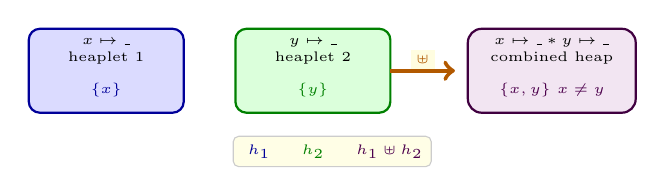
\begin{tikzpicture}[scale=0.82,font=\scriptsize]
\draw[fill=blue!14,draw=blue!60!black,thick,rounded corners=4pt] (0,0) rectangle (2.4,1.30);
\node[font=\tiny,align=center] at (1.20,0.95) {$x\mapsto\_$\\heaplet 1};
\draw[fill=green!14,draw=green!50!black,thick,rounded corners=4pt] (3.2,0) rectangle (5.6,1.30);
\node[font=\tiny,align=center] at (4.40,0.95) {$y\mapsto\_$\\heaplet 2};
\draw[->,ultra thick,orange!70!black] (5.6,0.65) -- (6.6,0.65) node[midway,above,font=\tiny,fill=yellow!12,inner sep=2pt] {$\uplus$};
\draw[fill=violet!10,draw=violet!50!black,thick,rounded corners=5pt] (6.8,0) rectangle (9.4,1.30);
\node[font=\tiny,align=center] at (8.10,0.95) {$x\mapsto\_ * y\mapsto\_$\\combined heap};
\node[font=\tiny,blue!60!black] at (1.20,0.35) {$\{x\}$}; \node[font=\tiny,green!50!black] at (4.40,0.35) {$\{y\}$}; \node[font=\tiny,violet!60!black] at (8.10,0.35) {$\{x,y\}$ $x\neq y$};
\node[font=\tiny,align=left,fill=yellow!10,draw=gray!40,rounded corners=2pt,inner sep=3pt] at (4.7,-0.60) {\textcolor{blue!60!black}{$\blacksquare$ $h_1$} \quad \textcolor{green!50!black}{$\blacksquare$ $h_2$} \quad \textcolor{violet!60!black}{$\blacksquare$ $h_1\uplus h_2$}};
\end{tikzpicture}
\caption{Separating conjunction $*$ as disjoint union: $x\mapsto\_$ and $y\mapsto\_$ occupy separate cells, so $x\mapsto\_ * y\mapsto\_$ forces $x\neq y$. The heap is the sum of its heaplets.}
\label{fig:sep-star}
\end{figure}

\begin{figure}[h]\centering
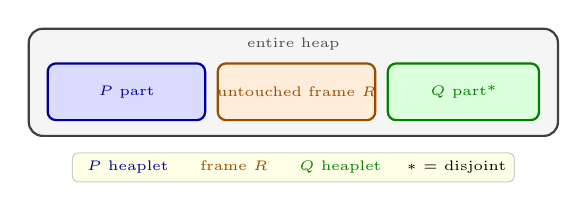
\begin{tikzpicture}[scale=0.80,font=\scriptsize]
\draw[fill=gray!08,draw=gray!50!black,thick,rounded corners=5pt] (0,0) rectangle (8.4,1.70);
\node[font=\tiny,gray!60!black] at (4.2,1.45) {entire heap};
\draw[fill=blue!14,draw=blue!60!black,thick,rounded corners=3pt] (0.3,0.25) rectangle (2.8,1.15);
\node[font=\tiny,blue!60!black] at (1.55,0.70) {$P$ part};
\draw[fill=orange!14,draw=orange!60!black,thick,rounded corners=3pt] (3.0,0.25) rectangle (5.5,1.15);
\node[font=\tiny,orange!60!black] at (4.25,0.70) {untouched frame $R$};
\draw[fill=green!14,draw=green!50!black,thick,rounded corners=3pt] (5.7,0.25) rectangle (8.1,1.15);
\node[font=\tiny,green!50!black] at (6.90,0.70) {$Q$ part*};
\node[font=\tiny,align=left,fill=yellow!10,draw=gray!40,rounded corners=2pt,inner sep=3pt] at (4.2,-0.50) {\textcolor{blue!60!black}{$\blacksquare$ $P$ heaplet} \quad \textcolor{orange!60!black}{$\blacksquare$ frame $R$} \quad \textcolor{green!50!black}{$\blacksquare$ $Q$ heaplet} \quad $*$ = disjoint};
\end{tikzpicture}
\caption{Frame intuition: prove $\{P\}\,C\,\{Q\}$ on its footprint; any disjoint frame $R$ stays untouched, so $\{P*R\}\,C\,\{Q*R\}$ holds. $*$ makes local reasoning sound.}
\label{fig:frame-heap}
\end{figure}

\begin{example}[* vs $\land$]
$x\mapsto3 * y\mapsto4$ implies $x\neq y$ and heap has exactly two cells. $x\mapsto3\land y\mapsto4$ on a two-cell heap with $x\neq y$ also holds, but on a one-cell heap with $x=y=5$ and content $3$ (and $4$? impossible—one cell cannot be both 3 and 4, so $\land$ still fails for that reason). The key difference: $x\mapsto\_ * y\mapsto\_$ \emph{forces} two cells; $x\mapsto\_\land y\mapsto\_$ does not force disjointness in the logic, but for singletons both happen to force distinctness because one cell cannot satisfy both points-to simultaneously unless contents equal.
\end{example}

% ============================================================
\section{Heap Axioms and the Frame Rule}
\label{sec:axioms}
Heap commands (with store $x,y$ and heap $h$):

\textbf{Lookup:} $\{x\mapsto\_\}\;y:=[x]\;\{y=v\land x\mapsto v\}$ where $v$ is the old content.

\textbf{Mutate:} $\{x\mapsto\_\}\;[x]:=e\;\{x\mapsto e\}$.

\textbf{New:} $\{\text{emp}\}\;x:=\text{new}(e)\;\{x\mapsto e\}$ (allocates fresh address).

\textbf{Dispose:} $\{x\mapsto\_\}\;\text{dispose}(x)\;\{\text{emp}\}$.

The star of the show is the \emph{frame rule}:
\[
\frac{\{P\}\,C\,\{Q\}}{\{P*R\}\,C\,\{Q*R\}}\ \text{provided }C\text{ does not modify free vars of }R.
\]
If $C$ is correct on its footprint $P$, it remains correct in any larger heap that adds a disjoint $R$—because $C$ never touches outside its footprint. This is \emph{local reasoning}: prove the small heap, get the big heap for free.

\begin{lstlisting}[language=C, caption={Heap axioms in C-like syntax: lookup, mutate, alloc. $*$ keeps footprints disjoint.}, label={lst:heap-axioms}]
// { x |-> _ }   x points somewhere
y = *x;         // { x |-> v && y==v }  y gets heap content v
// { x |-> _ }
*x = 3;         // { x |-> 3 }          heap cell updated
// { emp }
x = malloc(1); *x = 5; // { x |-> 5 }  fresh cell
free(x);        // { emp }              back to empty
\end{lstlisting}

\begin{lstlisting}[language=Python, caption={Modelling $*$ as disjoint dict union: $P*Q$ holds iff heap splits.}, label={lst:star-py}]
def sep_conj(P, Q, heap):
    """Check P*Q on heap (dict addr->val) by searching split."""
    addrs = list(heap.keys())
    from itertools import combinations
    for r in range(len(addrs)+1):
        for left_addrs in combinations(addrs, r):
            h1 = {a:heap[a] for a in left_addrs}
            h2 = {a:heap[a] for a in addrs if a not in left_addrs}
            if P(h1) and Q(h2):
                return True
    return False
# P = "x|->0": heap {x:0}; Q = "y|->0": heap {y:0}
# P*Q needs heap {x:0,y:0} with x!=y
\end{lstlisting}

% ============================================================
\section{Lists and Local Reversal}
\label{sec:lists}
Define $\text{ls}(x,y)$: linked list segment from $x$ to $y$ (where $y$ is null or another pointer). Inductive: $\text{ls}(x,x)\equiv\text{emp}$ (empty) and $\text{ls}(x,y)\equiv\exists n.\,x\mapsto n * \text{ls}(n,y)$ when $x\neq y$. Then full list $\text{list}(x)\equiv\text{ls}(x,\text{null})$.

\textbf{Reversal sketch:} $\{\text{list}(p)\}\; r:=\text{null};\texttt{while }p\neq\text{null}\texttt{ do }(n:=[p+1];[p+1]:=r;r:=p;p:=n)\;\{\text{list}(r)\land\text{list}(p)\equiv\text{original reversed}\}$. Invariant: $\text{ls}(r,\text{null}) * \text{ls}(p,\text{null})$ where the two segments are exactly the reversed prefix and the unprocessed suffix, and together they partition the original heap. Frame rule lets each iteration reason only about $p\mapsto n$ and $r$'s head.

\begin{example}[Two heaplets, one invariant]
Before iteration: heap $= \underbrace{r\mapsto\cdots *\cdots}_{reversed} * \underbrace{p\mapsto n * \text{ls}(n,\text{null})}_{suffix}$. Iteration swings $p$'s next to $r$, so new $r' = p$ and new $p' = n$. The invariant re-establishes as $\text{ls}(p',\text{null})$ is the tail and $\text{ls}(r',\text{null})$ is the grown reversed prefix. $*$ guarantees the prefix and suffix never share a cell, so the swing cannot create a cycle.
\end{example}

% ============================================================
\section{Magic Wand and Iterated Star}
\label{sec:wand}
$P -* Q$ is for ``if you give me a $P$-heap, together we make $Q$''. It is the right adjoint to $*$: $(P*Q\Rightarrow R)$ iff $(P\Rightarrow Q -* R)$. Intuition: $Q -* R$ is the ``heap remainder'' needed to go from $Q$ to $R$. Example: $(x\mapsto\_) -* (x\mapsto3)$ is the claim ``adding a heaplet where $x$ holds whatever is required to make $x\mapsto3$''—essentially an update promise.

Iterated $*$ describes arrays: $\circledast_{i=0}^{n-1} a+i\mapsto\_$ means $n$ disjoint cells at $a,\dots,a+n-1$. This lets specs of \texttt{memcpy} stay local: $\{\circledast_{i<n} src+i\mapsto v_i * \circledast_{i<n} dst+i\mapsto \_\}\;\texttt{memcpy}(dst,src,n)\;\{\circledast_{i<n} src+i\mapsto v_i * \circledast_{i<n} dst+i\mapsto v_i\}$. Without $*$, aliasing between $src$ and $dst$ would make the spec unsound; with $*$, $src\neq dst$ and non-overlapping are enforced structurally.

\begin{remark}[$*$ owns, $\land$ shares]
Think $*$ as ``owns disjointly'' and $\land$ as ``shares aliased view''. Ownership is what makes frame sound: you can frame only what you do not own in $P$. This is why Rust's borrow checker and separation logic's $*$ feel similar—both track disjoint ownership.
\end{remark}

% ============================================================
\section{Why Frame Prevents Leaks and Double-Free}
\label{sec:frame-safety}
Separating conjunction also tracks \emph{resource accounting}. $x\mapsto\_ * y\mapsto\_$ says there are exactly two cells owned; after $\text{dispose}(x)$ you own $y\mapsto\_$ alone—$x$'s cell is gone. Double-free $\{x\mapsto\_\}\;\text{dispose}(x);\,\text{dispose}(x)$ fails: after first dispose you own $\text{emp}$, so second dispose's pre $x\mapsto\_$ cannot be satisfied—no frame can rescue it because $\text{emp} * x\mapsto\_$ would require a fresh $x$ cell you do not own.

Leak detection is dual: $\{x\mapsto3\}\;\texttt{skip}\;\{\text{emp}\}$ is unprovable because $\text{emp}$ demands no cells but you still own $x\mapsto3$; no $*$ manipulation discards owned heap. This is how separation logic verifiers (Infer) catch leaks at compile time: owned heap that is not freed is a $*$ remainder that never reaches $\text{emp}$.

\begin{remark}[Garbage collection]
In GC languages, dispose is implicit and the post of dropping a reference is not $\text{emp}$ but a weaker ``garbage may remain''. Separation logic adapts by treating GC as an implicit frame: collected cells move to an invisible $R$ that the spec need not mention. The $*$ still forces disjointness before collection.
\end{remark}

% ============================================================
\section{Exercises}
\label{sec:ch07-exercises}
\begin{enumerate}[label=E7.\arabic*, leftmargin=*, itemsep=0.6em]
    \item \textbf{Alias vs $*$.} Show $x\mapsto0 * y\mapsto0\Rightarrow x\neq y$ but $x\mapsto0\land y\mapsto0$ does not imply $x\neq y$ on a heap where maps are sets? Explain via $*$'s split definition.
    \item \textbf{Mutate with frame.} From $\{x\mapsto\_*R\}\, [x]:=3 \,\{x\mapsto3*R\}$ derive why $R$ is untouched; give $R\equiv y\mapsto4$ and show the post still claims $y\mapsto4$.
    \item \textbf{List emp base.} Prove $\text{ls}(x,x)\equiv\text{emp}$ and $\text{ls}(x,y) * \text{ls}(y,z)\Rightarrow \text{ls}(x,z)$ by induction on length.
    \item \textbf{Dispose spec.} State $\{x\mapsto v * R\}\,\text{dispose}(x)\,\{R\}$ using frame; why is $*$ needed rather than $\land$?
    \item \textbf{Reversal invariant picture.} Draw heaplets before and after one iteration of in-place reversal, labelling $p$, $r$, $n$ and shading $*$ footprints blue/green with untouched suffix grey.
\end{enumerate}

\section*{Chapter Notes}
Reynolds (2002) and O'Hearn--Pym introduced separation logic; ``Separation Logic: A Logic for Shared Mutable Data Structures'' is the classic. For lists see Reynolds Ch.~1--2, Yang and Birkedal notes. Frame rule as local reasoning is O'Hearn's key insight; modern tools are Infer, VeriFast, and Viper.

\smallskip
\begin{remark}[Scaling to concurrency]
The same $*$ that gives frame for sequential heaps gives \emph{concurrent} separation logic's resource sharing: $P * Q$ can be split between threads with no race on owned cells. This is why separation logic became the foundation for verified concurrent data structures—ownership as logic. See O'Hearn's Concurrent Separation Logic (2007) for the direct extension.
\end{remark}

\smallskip
\begin{remark}[Mental model]
Draw every heap assertion as coloured boxes that cannot overlap if joined by $*$. If you can shade the heaplet of each $*$ conjunct with a distinct colour without overlap, the assertion is plausible; if two conjuncts demand the same cell with different contents, it is $\text{false}$.
\end{remark}
% End of Chapter 7
